\documentclass{article}
\usepackage{caption}
\usepackage{subcaption}
\usepackage{graphicx}
\usepackage{tikz}
\usepackage{tikzsymbols}
\usetikzlibrary{calc}
\usepackage{float}
\usepackage{pdflscape}
\usepackage{geometry}
\geometry{a4paper, landscape, margin=1cm}
\pagestyle{empty}

\def\centerarc[#1](#2)(#3:#4:#5){\draw[#1] ($(#2)+({#5*cos(#3)},{#5*sin(#3)})$) arc (#3:#4:#5);}

\begin{document}
	\centering
	\begin{figure}[H]
			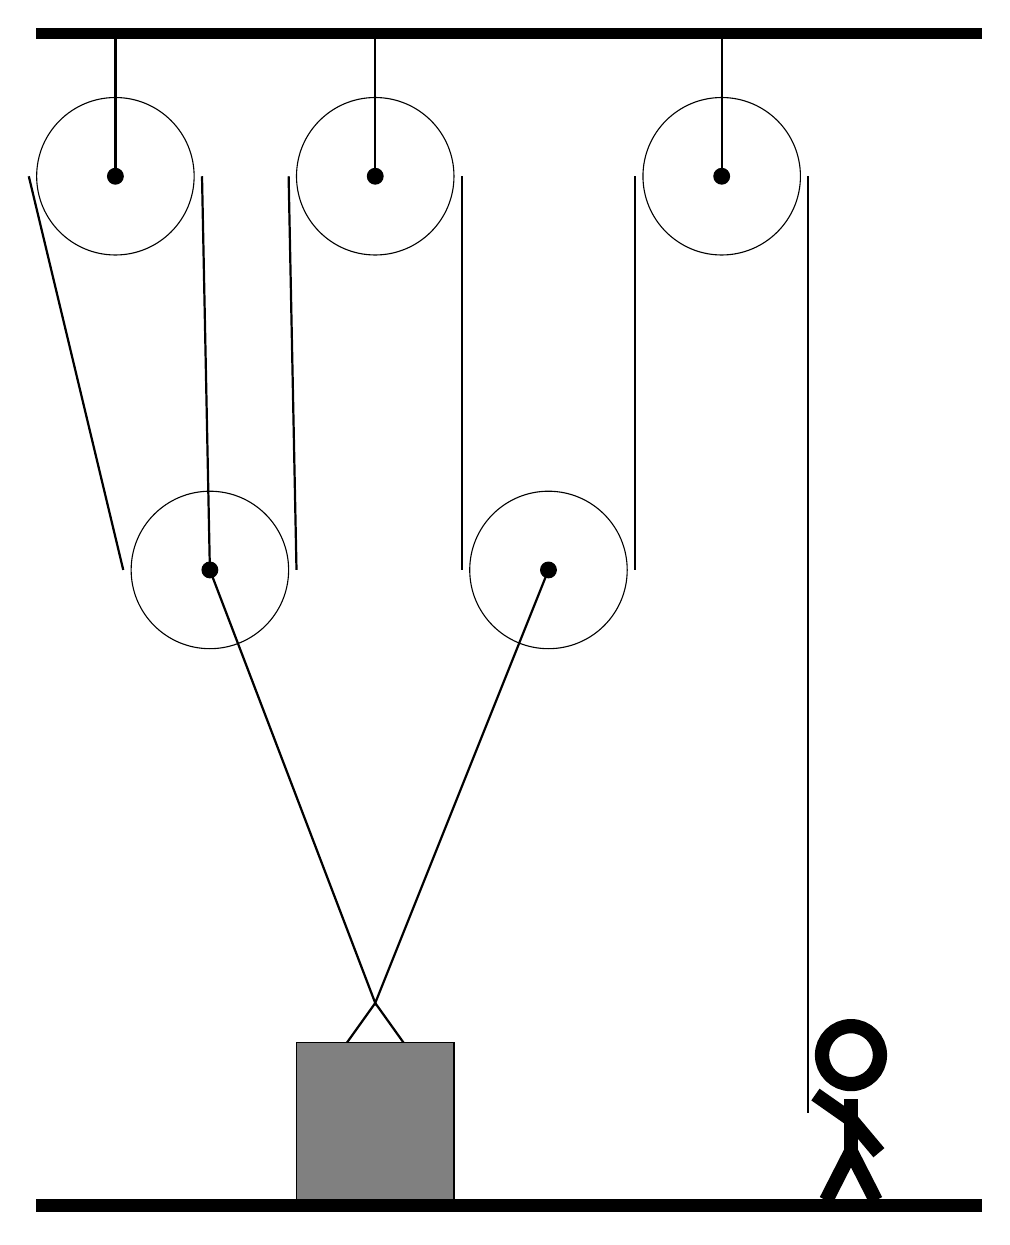
\begin{tikzpicture}
				%%%%% START %%%%%
								
				\draw[fill=black] (-2, 11.75) rectangle (10, 11.88);
				
				\draw (-1, 10) circle (1);
				\draw[fill=black] (-1, 10) circle (0.1);
				\draw[thick] (-1, 10) -- (-1, 11.75);
				
				\draw (2.3, 10) circle (1);
				\draw[fill=black] (2.3, 10) circle (0.1);
				\draw[thick] (2.3, 10) -- (2.3, 11.75);
				
				\draw (6.7, 10) circle (1);
				\draw[fill=black] (6.7, 10) circle (0.1);
				\draw[thick] (6.7, 10) -- (6.7, 11.75);
				
				\draw (0.2, 5) circle (1);
				\draw[fill=black] (0.2, 5) circle (0.1);
				
				\draw (4.5, 5) circle (1);
				\draw[fill=black] (4.5, 5) circle (0.1);
				
				\draw[thick] (0.2, 5) -- (2.3, -0.5)  -- (4.5, 5);
				\draw[thick]  (1.8, -1.2) -- (2.3, -0.5) -- (2.8, -1.2);
				\draw[fill=black!50] (1.3, -1.0) rectangle (3.3, -3.0);
				
				\draw[thick] (0.2, 5) -- (0.1, 10);
				\centerarc[thick](-1, 10)(0:180:1.1);
				\draw[thick] (-2.1, 10) -- (-0.9, 5);
				\centerarc[thick](0.2, 5)(180:360:1.1);
				\draw[thick] (1.3, 5) -- (1.2, 10);
				\centerarc[thick](2.3, 10)(0:180:1.1);
				\draw[thick] (3.4, 10) -- (3.4, 5);
				\centerarc[thick](4.5, 5)(180:360:1.1);
				\draw[thick] (5.6, 5) -- (5.6, 10);
				\centerarc[thick](6.7, 10)(0:180:1.1);
				\draw[thick] (7.8, 10) -- (7.8, -1.9);
				
				\node at (8.3, -1.9) {\Strichmaxerl[10][-35][-50]};
				
				\draw[fill=black] (-2, -3) rectangle (10, -3.15);
				%%%%% END %%%%%
			\end{tikzpicture}
	\end{figure}	
\end{document}